\mychapter{Implementações}
\label{Cap:implementacoes}

A aplicação desenvolvida envolve a comunicação entre o CLP WEG TPW-03, o microcontrolador NOVUS N2000 e o \textit{software} de teste desenvolvido no Elipse SCADA. Os sensores serão fisicamente ligados ao CLP e ao controlador da NOVUS. Para que os valores desses elementos sejam observados pelo sistema supervisório, há a necessidade de se estabelecer a comunicação entre todos os elementos.

Como o trabalho é baseado nas instalações físicas nos laboratórios do LAMP, é necessário que um total de 17 sensores de temperatura e dois de pressão sejam lidos pelo sistema final descrito no item 2.1 desse trabalho. A fim de tornar os testes mais rápidos e simples de serem executados, foram utilizados apenas dois sensores de temperatura (PT100). Visto que a lógica de obtenção de dados dos sensores é similar tanto para somente um, quanto para um valor $N>1$ de sensores, o fato de se utilizar apenas dois sensores não compromete o objetivo final de comunicar todos os 19 sensores do sistema de simulação de poços petrolíferos do LAMP.

\section{Comunicação}
Para haver uma leitura dos sinais dos sensores através do TPW-03, há a necessidade da conexão de módulos analógicos, uma vez que o módulo padrão do TPW-03 60HT-A não dispõe dessas entradas. Devido a isso, optou-se por utilizar o módulo de expansão do tipo 8AD. Esse módulo comporta oito entradas analógicas, sendo possível a leitura de até oito sensores cada. Para um projeto que precise utilizar mais de oito sensores, até 60 canais de entradas e 10 canais de saídas analógicas podem ser expansíveis ao módulo básico do TPW-03 (para o modelo 60H) utilizando mais módulos AD.

A Figura \ref{fig:ArquiteturaComunicacao} demonstra a arquitetura da rede de comunicação do sistema considerado nesse trabalho.

\begin{figure}[h!]
  \center
  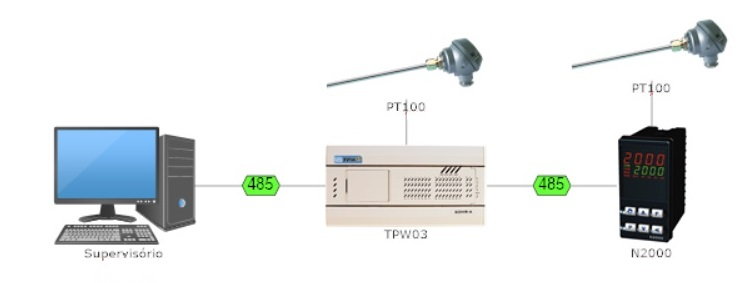
\includegraphics[scale=0.9]{ArquiteturaComunicacao.jpg}
  \label{fig:ArquiteturaComunicacao}
  \caption{Arquitetura da Aplicação.}
\end{figure}


A interligação dos sensores ao TPW-03 é feita segundo o manual de instalação do CLP \cite{weg2010manualinstalacao}. A Figura 3.2 apresenta o sistema de ligação de dispositivos externos, ao controlador. De acordo com o esquema de ligação apresentado, deve-se conectar o sensor à fonte de alimentação chaveada (utilizou-se uma fonte do tipo PSS24-W/2.5, 24Vdc 60W da WEG). Esse esquema de ligação é disponibilizado pelo próprio fabricante.

Como era necessária a conexão de apenas um sensor de temperatura (PT100) utilizou-se apenas o primeiro canal AD. Assim, em resumida explicação, conecta-se o polo positivo do PT100 à saída de tensão positiva da fonte de alimentação, o polo negativo do sensor ao pino A0 da expansão analógica do CLP, e a saída negativa da fonte de alimentação conecta-se ao pino C0 da expansão do controlador.

\begin{figure}[h!]
\centering
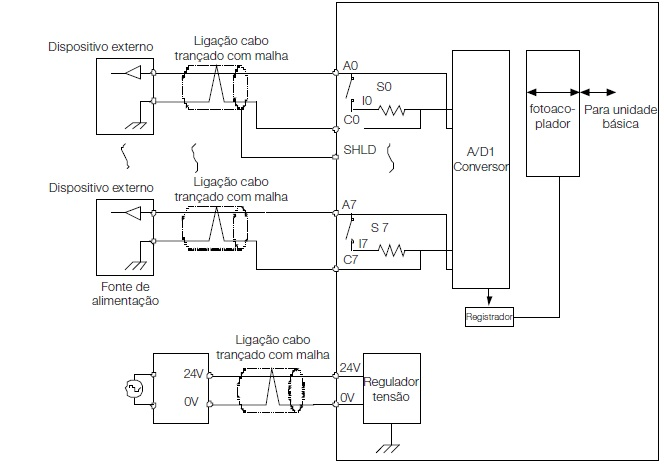
\includegraphics[scale=0.9]{Ligacao.jpg}
\label{fig:LigacaoAnalogico}
\caption{Especificação de ligação de dispositivos externos ao módulo de expansão TPW-03 8AD.}
\end{figure}


Para que ocorra a ligação do sensor PT100 com o microcontrolador da NOVUS, para o caso de sinais de corrente de 4 - 20mA, o fabricante indica a conexão apresentada na Figura \ref{fig:LigacaoNovus}. O pino positivo do PT100 é ligado ao pino 17 do N2000; o negativo do PT100 liga-se ao pino 22 do microcontrolador; e liga-se o pino 18 do aparelho da NOVUS ao seu pino 24.

\begin{figure}[h!]
\centering
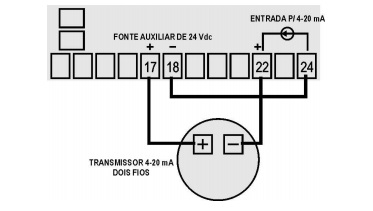
\includegraphics[scale=1.0]{LigacaoNovus.jpg}
\caption{Especificação de ligação de dispositivos externos ao N2000 do tipo 4 - 20mA.} \cite{novus2014folheto}
\label{fig:LigacaoNovus}
\end{figure}

\subsection{Protocolo de Comunicação}

Uma vez interligados os sensores aos controladores, há a necessidade da comunicação entre ambos, juntamente com o PC. Essa comunicação é feita de maneira serial via RS-485 utilizando o protocolo Modbus modo RTU, discutido no capítulo 2. A razão da escolha desse protocolo para interligação dos elementos do sistema se deu pela sua popularidade, eficiência, confiabilidade e facilidade de implementação no Elipse SCADA.

A implementação do protocolo Modbus no software da Elipse se dá através de um \textit{driver} Modbus da própria \textit{Elipse software}, disponível para \textit{download} no próprio site da empresa. O software que comporta esse \textit{driver} funciona sempre como mestre de uma rede Modbus, o que define o PC como o mestre da comunicação e \textit{host} da aplicação SCADA.

O \textit{driver} da Elipse foi desenvolvido utilizando uma biblioteca chamada IOKit, responsável por implementar a camada física, definindo parâmetros como: porta de comunicação, \textit{baud rate}, bits de dado, paridade e bits de parada (para uma comunicação serial) \cite{iokit2009manual}. 

\section{Configurações dos parâmetros do WEG TPW-03}

O TPW-03 modelo 60HT-A possui três portas de comunicação: porta de comunicação do PC; cartão de expansão TPW-03 232RS e TPW-03 485RS; e porta de comunicação RS485. Das três, utilizou-se a primeira e a última durante os experimentos descritos nesse trabalho. Para estabelecer a comunicação via porta do PC, utiliza-se um cabo serial conectado via USB ao computador.

Essa comunicação permite realizar Download/Upload de programas em LADDER e conexão do CLP como escravo Modbus. A comunicação do CLP com o PC por essa porta deve ser estabelecida através do software da WEG: TPW03-PCLINK. Nesse software, é possível selecionar a ferramenta de conexão e se estabelecer o link entre o dispositivo e o PC conforme a Figura \ref{fig:link}.

\begin{figure}[h!]
\centering
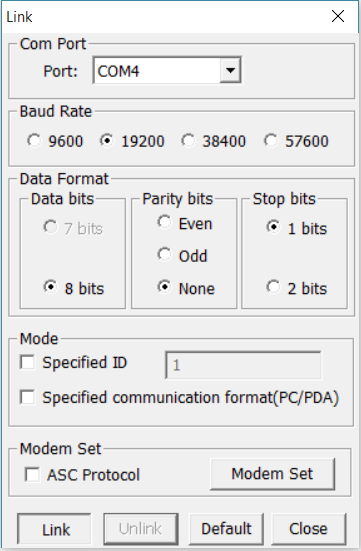
\includegraphics[scale=0.7]{link.png}
\caption{Link do CLP com o PC via TPW03-PCLINK}
\label{fig:link}
\end{figure}

Nessa conexão define-se um \textit{baud rate} de 19200, visto que é o \textit{baud rate} padrão para as três portas \cite{weg2010manualinstalacao}[p.29]. Definiu-se dados no formato de 8 bits, sem paridade e 1 bit de parada. Esses parâmetros poderiam ser alterados contanto que os mesmos parâmetros sejam definidos em todos os dispositivos que se conectam na rede Modbus. É necessário também definir a porta de comunicação em que o CLP está conectado. No exemplo em questão, a conexão era estabelecida na COM4.

Após feito o link, é necessário programar o formato de comunicação e o \textit{baud rate} no registro especial da comunicação no CLP. Para isso, o endereço D8321 deve ser configurado com um valor correspondente à comunicação desejada. Esse registrador é definido especialmente para indicar parâmetros como o comprimento de dados, bit de paridade, \textit{stop bit} e \textit{baud rate} de acordo com a Figura \ref{fig:portaPC}.

\begin{figure}[h!]
\centering
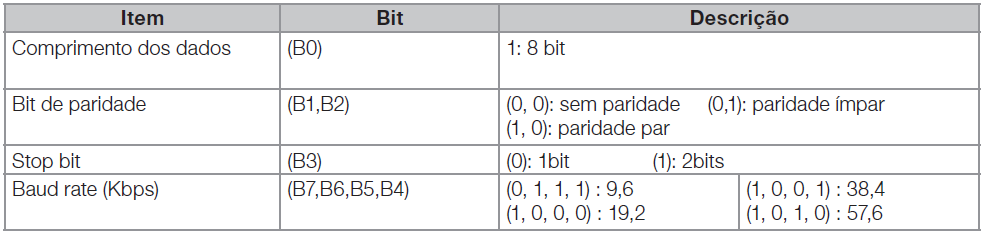
\includegraphics[scale=0.7]{portaPC.png}
\caption{Programação de comunicação para a porta do PC ($D8321$)}\cite{weg2010manualinstalacao}[p.30].
\label{fig:portaPC}
\end{figure}

Considerando os parâmetros desejados, deve-se passar o valor binário de $10000001$ para o registrador $D8321$, isso corresponde ao valor 81 em hexadecimal. Esse valor hexadecimal é movido para esse registrador na programação em LADDER (Figura \ref{fig:LadderComunicacao}). 

\begin{figure}[h!]
\centering
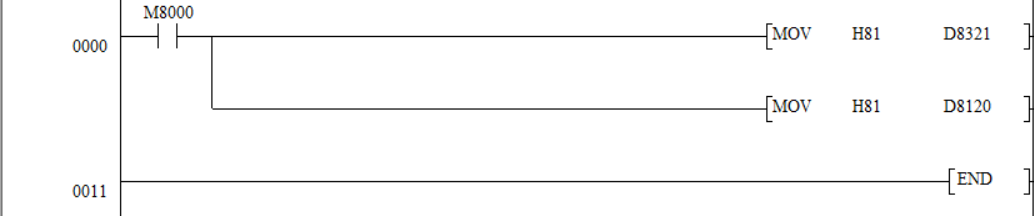
\includegraphics[scale=0.65]{ladderComunicacao.png}
\caption{Programação em LADDER para configuração de comunicação.}
\label{fig:LadderComunicacao}
\end{figure}

No mesmo programa é possível definir os parâmetros para comunicação via RS485. Para isso, deve-se configurar o registrador $D8120$ com os parâmetros desejados conforme a Figura \ref{fig:rs485}. Como deseja-se os mesmos parâmetros de comunicação, a configuração permanece a mesma, dessa forma, o valor 81 hexadecimal também deve ser passado para o registrador $D8120$.

\begin{figure}[h!]
\centering
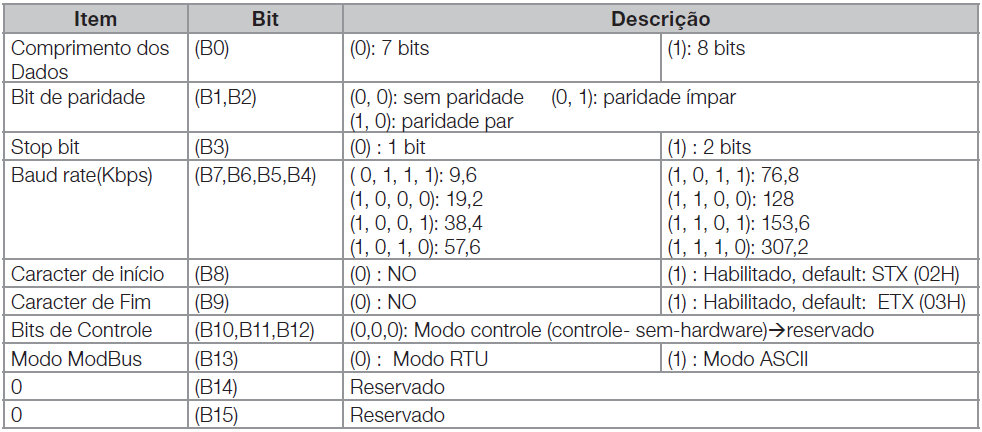
\includegraphics[scale=0.7]{rs485.png}
\caption{Programação do formato de comunicação para RS485 (D8120)}\cite{weg2010manualinstalacao}
\label{fig:rs485}
\end{figure}

Feita a programação em LADDER, realiza-se o download do programa para o CLP da WEG e o link com o software TPW03-PCLINK pode ser desfeito através da mesma ferramenta descrita na Figura \ref{fig:link}.

\subsection{Configuração do módulo 8AD}

Para que o módulo de expansão analógica 8AD funcione corretamente de acordo com a aplicação desejada, é necessário programar a memória do sistema para que o mesmo atue corretamente sobre as unidades conectadas à ele. Essa programação é feita de acordo com a Figura \ref{fig:memoria8AD} com informações do fabricante.

\begin{figure}[h!]
\centering
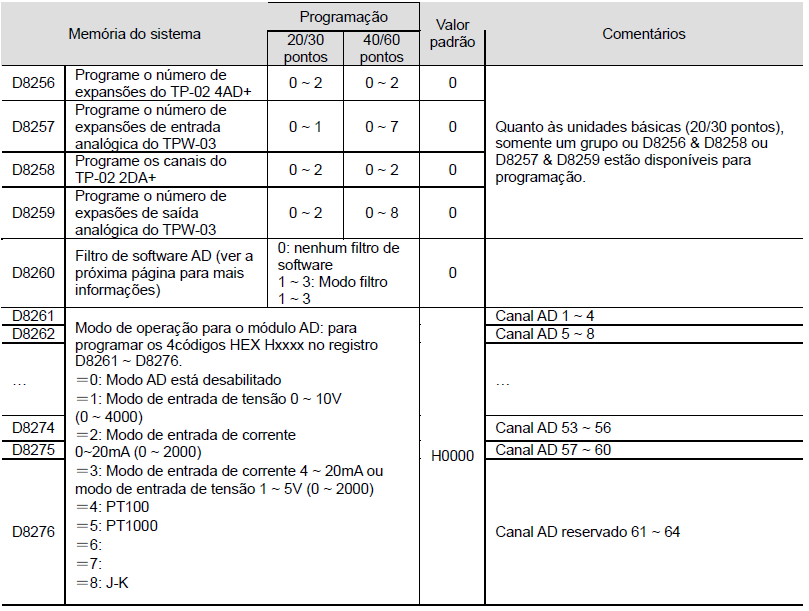
\includegraphics[scale=0.7]{memoria8AD.png}
\caption{Configuração do Modo de operação do módulo 8AD.}\cite{weg2010manualinstalacao}[p.64]
\label{fig:memoria8AD}
\end{figure}

Através do TPW03-PCLINK, configura-se os registradores ($D8256$ à $D8276$) com os valores desejados de operação do módulo. Na aplicação desenvolvida nesse trabalho, deseja-se apenas um módulo e que este opere em modo de entrada de corrente 4 - 20mA.    Para isso, deve-se passar o valor decimal $K = 1$ para o registrador $D8257$ que indica o número de expansões analógicas do TPW03. Além disso, o valor hexadecimal 3 deve ser movido para o registrador correspondente aos canais analógicos que serão utilizados.

Conforme a figura \ref{fig:Config8AD} indica, foi passado o valor '$H3333$' para o registrador $D8261$ para que as 4 primeiras entradas da expansão fossem habilitadas para leitura dos sensores no modo de operação 4-20mA.

\begin{figure}[h!]
\centering
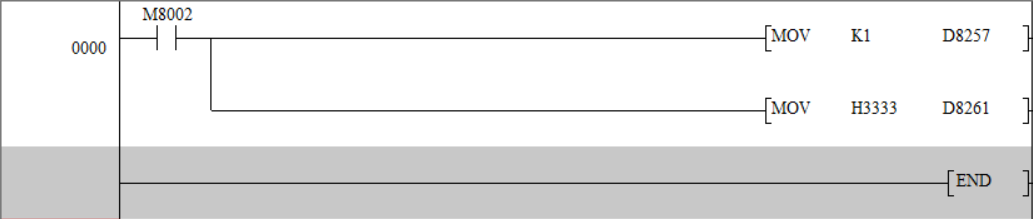
\includegraphics[scale=0.68]{Config8AD.png}
\caption{Programação em LADDER para configuração do módulo 8AD.}
\label{fig:Config8AD}
\end{figure}

Observa-se também que o modo de operação 4 também indica a leitura específica de um aparelho PT100. Teoricamente, essa forma de operação também deve servir para os mesmos propósitos desejados aqui, porém os testes com essa forma de operação não foram realizados. A escolha do modo de operação 4-20mA em detrimento do modo PT100 foi feita para que caso se deseje conectar outro tipo de sensor que atue de 4-20mA ao CLP, este já esteja devidamente configurado para receber o aparelho.




\section{Configuração dos parâmetros do NOVUS N2000}

O controlador da NOVUS é capaz de se comunicar com o PC de maneira serial via RS485, também utilizando protocolo Modbus RTU. Para configurar a comunicação serial nesse controlador, deve-se alterar os valores das variáveis $bAud$ e $Addr$. Como deseja-se que todos os integrantes da comunicação tenham o mesmo \textit{baud rate} e configuração de bits, configura-se o $bAud$ com o valor 4, o que corresponde a um \textit{baud rate} de 19200, conforme indicado na tabela de registradores para comunicação serial do produto \cite{novus2014modbus}. O parâmetro $Addr$ corresponde ao identificador do controlador na rede Modbus. Nesse caso, conforme discute-se posteriormente, considera-se o N2000 como o segundo escravo da rede Modbus, atribuindo-se $Addr = 2$. A manipulação desses parâmetros do N2000 é realizada no próprio controlador, sem a necessidade de um software externo.

\section{Comunicação com o Sistema Supervisório}

Como mencionado na no item 3.1.1, a comunicação dos dois controladores com o PC se dá através do \textit{driver} Modicon Modbus em sua versão v3.19 (IOKitLib v2.054), permitindo com que a aplicação desenvolvida no Elipse se comunique com qualquer dispositivo escravo que implemente o protocolo Modbus.

Os parâmetros de comunicação Modbus podem ser configurados através do \textit{Organizer} dentro do Elipse SCADA. Seleciona-se o \textit{Driver Modbus} e na aba de opções \textit{Extras}, define-se o modo de aplicação (\textit{RTU Mode}) e com \textit{Data Address Model Offset = 0} visto que o endereçamento das memórias dos controladores utilizados iniciam-se de 0. Na aba \textit{Operations}, define-se as operações de leitura e escrita que podem ser utilizadas. Na aba \textit{Setup}, define-se a camada física (Serial para essa comunicação) e dependendo da opção escolhida nessa aba, configura-se a comunicação nas abas subsequentes. Para o caso de uma comunicação serial, define-se a porta de comunicação, o \textit{Baud Rate}, \textit{Data Bits}, \textit{Paridade} e \textit{Stop Bits}. Esses parâmetros são configurados com os mesmos valores discutidos anteriormente para os dois controladores.

Uma vez configurados os parâmetros de comunicação do TPW-03 e do N2000, pode-se fazer a ligação desses dispositivos com o Elipse SCADA e ter-se um sistema supervisório capaz de atuar sobre os controladores.




%aaaaaaaaaaaaaaaaaaaaaaaaaaaaaaaaaaaaaaaaaaaaaaaaaaaaaaaaaaaaaaaaaaaaaaaaaaaaaaaaaaaaaaaaaaaaaaaaaaaaaaaaaaaaaaaaaaaaaaaaaaaaaaaaaaaaaaaaaaaaaaaaaaaa












%ZZZZZZZZZZZZZZZZZZZZZZZZZZZZZZZZZZZZZZZZZZZZZZZZZZZZZZZZZZZZZZZZZZZZZZZZZZZZZZZZZZZZZZZZZZZZZZZZ

















